\documentclass[11pt]{article}
\usepackage[T1]{fontenc}
\usepackage[utf8]{inputenc}
\usepackage{amsmath,amssymb,amsthm,mathtools}
\usepackage[margin=1in]{geometry}
\usepackage{booktabs}
\usepackage{array}
\usepackage{microtype}
\usepackage{enumitem}
\usepackage[font=small,labelfont=bf]{caption}
\usepackage{graphicx}
\usepackage{xcolor}
\usepackage{tikz}
\usepackage{listings}
\setlength{\emergencystretch}{2.5em}
\usepackage[obeyspaces,spaces]{url}
\usepackage{hyperref}
\hypersetup{colorlinks=true, linkcolor=black, citecolor=black, urlcolor=blue}
\usepackage[capitalise,noabbrev]{cleveref}
\makeatletter\g@addto@macro\UrlBreaks{\do\-}\makeatother

\newtheorem{theorem}{Theorem}[section]
\newtheorem{proposition}[theorem]{Proposition}
\newtheorem{lemma}[theorem]{Lemma}
\newtheorem{corollary}[theorem]{Corollary}
\theoremstyle{definition}
\newtheorem{definition}[theorem]{Definition}
\newtheorem{remark}[theorem]{Remark}
\usepackage{etoolbox}
\AtBeginEnvironment{lemma}{\crefalias{theorem}{lemma}}
\AtBeginEnvironment{proposition}{\crefalias{theorem}{proposition}}
\AtBeginEnvironment{corollary}{\crefalias{theorem}{corollary}}
\AtBeginEnvironment{definition}{\crefalias{theorem}{definition}}
\AtBeginEnvironment{remark}{\crefalias{theorem}{remark}}

\DeclareUrlCommand\lean{\urlstyle{tt}}
\newcommand{\re}{\operatorname{Re}}
\newcommand{\C}{\mathbb{C}}
\newcommand{\R}{\mathbb{R}}
\newcommand{\N}{\mathbb{N}}
\newcommand{\Z}{\mathbb{Z}}
\newcommand{\Q}{\mathbb{Q}}
\newcommand{\OK}{\mathcal{O}_K}
\newcommand{\disc}{\operatorname{disc}}
\newcommand{\Nm}{\operatorname{N}}
\newcommand{\Cl}{\operatorname{Cl}}

% Draft markers.  \PENDING: a fact not yet available.  \PLACEHOLDER: an item only the author can supply.
% Both print in red; neither may survive into a release.
\newcommand{\PENDING}[1]{\textcolor{red}{[\textsc{pending}: #1]}}
\newcommand{\PLACEHOLDER}[1]{\textcolor{red}{[\textsc{author}: #1]}}

\definecolor{leanbg}{HTML}{F4F2EC}
\newenvironment{inlean}{\par\medskip\noindent
\begin{tikzpicture}\node[fill=leanbg,rounded corners=2pt,
  inner sep=6pt,text width=\dimexpr\linewidth-12pt\relax,font=\small]\bgroup\textbf{In Lean.}\ }%
  {\egroup;\end{tikzpicture}\par\medskip}

\lstdefinelanguage{Lean}{
  morekeywords={theorem,lemma,def,noncomputable,import,namespace,end,open,by,fun,sorry,example,variable,structure,where},
  sensitive=true, morecomment=[l]{--}, morecomment=[s]{/-}{-/}, morestring=[b]",
}
\lstset{language=Lean, basicstyle=\footnotesize\ttfamily, backgroundcolor=\color{leanbg},
  frame=single, framerule=0pt, framesep=4pt, xleftmargin=4pt, xrightmargin=4pt,
  breaklines=true, columns=fullflexible, keepspaces=true, showstringspaces=false,
  literate={ℝ}{{$\mathbb{R}$}}1 {ℂ}{{$\mathbb{C}$}}1 {ℕ}{{$\mathbb{N}$}}1 {ℤ}{{$\mathbb{Z}$}}1 {ℚ}{{$\mathbb{Q}$}}1
           {∀}{{$\forall$}}1 {∃}{{$\exists$}}1 {→}{{$\to$}}1 {≠}{{$\neq$}}1 {≤}{{$\le$}}1 {≥}{{$\ge$}}1
           {∈}{{$\in$}}1 {∑}{{$\sum$}}1 {‖}{{$\Vert$}}1 {¬}{{$\neg$}}1 {∧}{{$\wedge$}}1
           {α}{{$\alpha$}}1 {χ}{{$\chi$}}1 {σ}{{$\sigma$}}1 {π}{{$\pi$}}1 {·}{{$\cdot$}}1 {²}{{$^2$}}1}

\title{Explicit two-sided bounds for imaginary quadratic class numbers, kernel-checked: the $7/8$ quasi-Riemann hypothesis at real points, in Lean~4}
\author{Peter W. Murphy}
\date{November 2026 (v2.0.0)\\[2pt] \small Repository \url{https://github.com/DrMurphyIsIn/boundaries-of-class}, directory \lean{two-sided-bounds/}\\ \small DOI \url{https://doi.org/10.5281/zenodo.23924566} (v2.0.0)\\ \small (all versions: \url{https://doi.org/10.5281/zenodo.23550257})}

\begin{document}
\maketitle

\begin{abstract}
We prove in Lean~4 over Mathlib, and check with two independent kernels, explicit bounds for the class number $h$ of every imaginary quadratic field $K = \Q(\sqrt{-m})$ in terms of $d = |\disc K|$. The lower bounds are $h \ge \frac13\sqrt d/\log d$ for $d \ge 2981$ and $h \ge d^{7/16}/17$ for $d \ge 1000$. The upper bounds are Dirichlet's class number formula $L(1,\chi) = \pi h/\sqrt d$, $h \le \frac1\pi\sqrt d(\log d + \frac76)$, and the textbook $h \le \frac1\pi\sqrt d(\frac12\log d + \log(\log d + \frac13) + \frac53)$ from an explicit P\'olya--Vinogradov inequality. Inverted, the lower bounds say that $h(K) \le h$ forces $d \le \min\bigl(\max(1000, (17h)^{16/7}), \max(2981, (6h(\log 6h + \log(2\log 6h)))^2)\bigr)$. Ten explicit thresholds follow, from $h \le 1 \Rightarrow d < 660$ to $h \le 5000 \Rightarrow d < 6.32\cdot 10^{10}$, and three point values, among them $d \ge 2^{40} \Rightarrow h \ge 17{,}450$. All $28$ statements use only Mathlib's definitions. The lower bounds follow the class-sum extension of the Chowla--Selberg argument posted in the comments of Terence Tao's tenth-discriminant challenge, with one change: each ideal class is charged the exact minimum, over its leading coefficient, of its Chowla--Selberg main term, and a $K_{1/2}$ kernel bound controls the remainder. Their deep input is OpenAI's theorem that no Dirichlet $L$-function vanishes in $\re s > 7/8$. It enters through one edge of the checked closure, at real points only, and its Lean proof is inside that closure. The upper bounds use no zero-free region. As far as we know, among explicit bounds that use the $7/8$ input at real points only, posted or published by 21 October 2026 (the thread) and 23 October 2026 (the papers), the lower bounds improve on all others except at class number one, and at two points where our own evaluation of Jaswal's method, which he did not post, gives more. A bound from the full half-plane by Littlewood's method, posted in the repository zeta-lab, is weaker at every threshold we tabulate but overtakes ours for very large $d$; we record the crossovers. Comparator accepted all $28$ theorems under nanoda and Lean's kernel. A closure audit found only the three standard axioms, and a separate AI review session reproduced the whole run from its own copies with no differences. The mathematics is not new in kind: the lower bound is the Gronwall--Hecke deduction published by Landau in 1918, run with OpenAI's theorem, and the upper bounds are classical.
\end{abstract}

%=====================================================================================================
\section{Introduction}
%=====================================================================================================

\subsection{The theorems}

For an imaginary quadratic field $K$, write $d = |\disc K|$ and $h = h(K)$. The class number formula gives $h = \sqrt d\,L(1,\chi_{-d})/\pi$ for $d > 4$. Here $L(1,\chi_{-d})$ is at most of order $\log d$, and by Siegel's theorem it is at least of order $d^{-\varepsilon}$ for every $\varepsilon > 0$, so $h = d^{1/2+o(1)}$. The lower half of that statement, in its classical form, cannot be made effective. This paper proves explicit two-sided versions, by analytic routes that the Lean kernel has checked step by step.

\begin{theorem}[informal form of \cref{thm:main}]\label{thm:informal}
Let $K = \Q(\sqrt{-m})$ with $m \ge 1$ squarefree, and $d = |\disc K|$.
\begin{enumerate}[nosep]
\item[\textup{(L$'$)}] If $d \ge 2981$, then $h(K) \ge \frac13\sqrt d/\log d$.
\item[\textup{(P$'$)}] If $d \ge 1000$, then $h(K) \ge d^{7/16}/17$.
\item[\textup{(CNF)}] If $d \ge 5$, then $L(1,\chi) = \pi h(K)/\sqrt d$ for the character $\chi$ of $K$, and $L(1,\chi) = 2\pi h(K)/(w(K)\sqrt d)$ for every $d$.
\item[\textup{(U$'$)}] If $d \ge 5$, then $h(K) \le \frac1\pi\sqrt d\,(\log d + \frac76)$.
\item[\textup{(U$''$)}] If $d \ge 5$, then $h(K) \le \frac1\pi\sqrt d\,(\frac12\log d + \log(\log d + \frac13) + \frac53)$.
\item[\textup{(B$^*$)}] If $h(K) \le h$, then $d \le \min\bigl(\max(1000, (17h)^{16/7}),\ \max(2981, (A(\log A + \log(2\log A)))^2)\bigr)$, with $A = 6h$.
\item[\textup{(T)}] If $h(K) \le N$, then $d < X_N$, for the ten pairs $(N, X_N)$ of \cref{tab:thresholds}; and $d \ge 2\cdot10^9$, $1.98\cdot10^{10}$ or $2^{40}$ implies $h(K) \ge 1101$, $3007$ or $17{,}450$.
\end{enumerate}
\end{theorem}

The formal statement also contains the Pólya--Vinogradov inequality with an explicit constant, the bound $\|L(1,\chi)\| \le \log q + \frac76$ for every non-trivial character, the half-log bound for primitive characters, and the primitivity and uniqueness of the character of $K$ (\cref{sec:statement}).

\subsection{History}\label{sec:history}

\paragraph{From zero-free segments to class numbers.} A theorem of Gronwall and Hecke, published by Landau in 1918 \cite{Landau1918}, says that if the zeta function of $\Q(\sqrt{-d})$ has no zero on the real segment $\frac12 < s < 1$, then $h(-d)$ is at least of order $\sqrt d/\log d$. The deduction needs much less than the whole segment: a real zero-free interval of length about $1/\log d$ to the left of $s = 1$ already gives $L(1,\chi_{-d}) \gg 1/\log d$. Part (L$'$) is this deduction, with an explicit constant. What has changed is that its hypothesis now has a proof, OpenAI's, whose Lean version is kernel-checked although its manuscript has not been refereed.

\paragraph{Ineffective and logarithmic bounds.} Heilbronn proved Gauss's conjecture $h \to \infty$ in 1934 \cite{Heilbronn1934}. Siegel showed in 1935 \cite{Siegel1935} that $\log h \sim \log\sqrt d$, so $h \gg_\varepsilon d^{1/2-\varepsilon}$, with a constant no one can compute: the proof splits on whether an exceptional real zero exists. Tatuzawa \cite{Tatuzawa1951} made the bound effective for every discriminant with at most one exception. Goldfeld showed in 1976 \cite{Goldfeld1976} that an elliptic curve whose $L$-function vanishes to order three at the centre would give an effective bound growing like $\log d$; Gross and Zagier supplied the curve \cite{GrossZagier1986}, and Oesterlé made the constant explicit \cite{Oesterle1985}. As recalled in comment 698454 of Tao's thread \cite{Tao2026}, following Goldfeld's survey \cite{Goldfeld1985}, the constant is $1/7000$ in front of $\log d$, up to a factor depending on the prime divisors of $d$. Class numbers one and two had been settled earlier, by other methods \cite{Heegner1952,Baker1966,Stark1967,Baker1971,Stark1971}, and Watkins determined every field with $h \le 100$ \cite{Watkins2004}. The decomposition of $\zeta_K$ into Epstein zeta functions, one for each form class, each expanded in a Fourier series, is old in this problem: Montgomery and Weinberger used it \cite{MontgomeryWeinberger1974}, and Watkins's method evaluates a refinement of it at low-lying zeros of auxiliary $L$-functions \cite[\S3]{Watkins2004}. Watkins also recalls that the generalized Riemann hypothesis implies $h \ge (1 + o(1))(\pi/12e^\gamma)\sqrt d/\log\log d$ (Littlewood), and that this is best possible up to a factor of two (Paley) \cite[p.~908]{Watkins2004}.

\paragraph{October 2026.} OpenAI's openai/math repository \cite{OAImath} contains a manuscript and a Lean proof that no Dirichlet $L$-function vanishes in the half-plane $\re s > 7/8$, apart from the pole of the trivial character \cite{OAIqrh}, and a separate argument excluding Landau--Siegel zeros \cite{OAIsiegel}. Banks gave a detailed proof of the second with explicit constants \cite{Banks2026}, Kerr a simpler proof \cite{Kerr2026}, and Green another \cite{Green2026}. Kimura made the zero gap explicit, $(1-\beta)\log q \ge 5.8\cdot10^{-4}$, proved his thresholds for $|d_K|$ in Lean with two kernels, and determined all imaginary quadratic fields with $h \le 2000$ \cite{Kimura2026}. Jaswal, assuming Kimura's bound for real zeros, determined all fields with $h \le 3000$ \cite{Jaswal2026}. His key analytic tool is Hecke's integral representation of the Dedekind zeta function \cite{Hecke1917}, which gives $h \ge B(|D|, \beta)$ whenever $\zeta_K(\beta) \le 0$ \cite[Prop.~2.2]{Jaswal2026}, and with it $h > \sqrt{|D|}/(5\log|D|)$ for every $D$ \cite[Thm.~1.3]{Jaswal2026}.

Earlier, on 8 October, the repository zeta-lab posted, from the full half-plane and Littlewood's method, the bound $h \ge \sqrt{|D|}/(10\pi\log\log|D|)$ for every fundamental $D < -3$, and the list of fields with $h \le 1500$ \cite{ZetaLab2026}.

\paragraph{Tao's challenge.} On 20 October 2026 Tao posted a challenge \cite{Tao2026}: bound a hypothetical tenth discriminant of class number one without Heegner's method, with AI use allowed and disclosed. In the comments, michaelmross wrote down the Chowla--Selberg expansion of the principal form (comment 698466); Tao observed that with the $7/8$ theorem it gives $d < 655$ (comment 698471); and LemmaLab certified $d \le 653$ by evaluating it at $s = 7/8$ (comment 698472). LemmaLab then extended the argument to every class number (comment 698478): the Dedekind zeta function is half the sum of the Epstein zeta functions of the $h$ reduced forms, the expansion applies to each, and for every $s \in [7/8, 1)$
\[
h \ge \frac{2\zeta(2s)}{A(s)\,d^{1/2-s} + R(d,s)} .
\]
Optimizing $s$ and certifying in ball arithmetic, LemmaLab posted thresholds for every $h$: $h \le 2 \Rightarrow d \le 4164$, $h \le 100 \Rightarrow d \le 6.64\cdot10^7$, $h \le 2000 \Rightarrow d \le 5.42\cdot10^{10}$, and $d \ge 2^{40} \Rightarrow h \ge 7946$. In a second comment (698484), LemmaLab used the bound at $s = 7/8$ in the form $h \ge d^{3/8}/12$. A comment posted anonymously (698561) linked the paper of Jaswal cited above, and reported that under the $7/8$ assumption the class group tables of Mosunov and Jacobson, complete below $2^{40}$, would settle every class number up to $17{,}357$. That rests on $B(2^{40}, 7/8) = 17{,}357.92$, so $d \ge 2^{40} \Rightarrow h \ge 17{,}358$ \cite[Remark~4.2]{Jaswal2026}. We read the thread in a copy saved on 21 October 2026.

This paper is the fifth entry of a repository, \emph{The Boundaries of Class}, that collects our work on this question; its first four entries were released under the name tenth-discriminant \cite{TenthDisc}. They formalized the class number one argument \cite{CN1paper}, a determinant proof of class number one \cite{DETpaper}, and LemmaLab's extension for $h \le 2$ at $s = 7/8$ \cite{HCNpaper}, which we call the first, the determinant and the second paper, and surveyed the posted class-number-one bounds. This paper reuses the second paper's machinery unchanged. The sixth entry, a classification of the fields with $h \le 3500$ on Jaswal's method \cite{H3500paper}, is not kernel-checked; on its route under the $7/8$ input, the one analytic bound it needs is the point value at $2^{40}$ proved here.

\subsection{The route}\label{sec:route}

For $\re s > 1$,
\[
\zeta(s)L(s,\chi) = \zeta_K(s) = \sum_{C \in \Cl(K)} \tfrac12 Z_{Q_C}(s),
\]
where $Q_C$ is a positive definite form of discriminant $-d$ with leading coefficient $1 \le a_C \le \frac23\sqrt d$, and $a_C = 1$ for the principal class. The second paper's Chowla--Selberg formula writes each class sum, at real $\sigma \in (\frac12, 1)$, as
\[
g(a_C) + E_C(\sigma), \qquad g(a) = a^{-\sigma}\zeta(2\sigma) - K\,a^{-(1-\sigma)},
\]
with an explicit $K = K(d,\sigma) > 0$ and a remainder $E_C$ (\cref{sec:lower}). At $\sigma \ge 7/8$ the left side $\zeta(\sigma)L(\sigma,\chi)$ is at most zero, because $\zeta(\sigma) < 0$ and the $7/8$ theorem makes $L(\sigma,\chi) \ge 0$. LemmaLab's posted bound, like the first version of this work, charges every class the principal form's negative term $-K$ and keeps the positive term $a^{-\sigma}\zeta(2\sigma)$ for the principal class only. But $g$ has an exact minimum over $a > 0$, by Bernoulli's inequality, and that minimum is of size $d^{-\sigma/2}$, while $K$ is of size $d^{1/2-\sigma}$. Charging every non-principal class its minimum, and bounding the remainder by a $K_{1/2}$ kernel bound, gives
\[
h \ge 1 + \frac{P(d,\sigma)}{m(d,\sigma)}, \qquad m(d,\sigma) \asymp d^{-\sigma/2}.
\]
At $\sigma = 7/8$ this raises the exponent from LemmaLab's $3/8$ to $7/16$, and near $\sigma = 1$ it roughly doubles the constant, to $2\zeta(2)/(\pi e) \approx 0.385$ as $d \to \infty$. Every lower bound of \cref{thm:informal} comes from this inequality, at $\sigma = 7/8$ or at $\sigma = 1 - 2/\log d$, with rational brackets. The upper bounds come from a different, classical route: Mathlib's residue formula for $\zeta_K$ gives the class number formula, and partial summation, with or without the Pólya--Vinogradov inequality, bounds $L(1,\chi)$.

\subsection{What is new here, and what is not}\label{sec:positioning}

\begin{itemize}
\item \textbf{The mathematics is not new in kind.} (L$'$) is the Gronwall--Hecke deduction with OpenAI's theorem as input. The class-sum route is LemmaLab's. The upper bounds are Dirichlet's formula, partial summation and the inequality of Pólya and Vinogradov \cite{Dirichlet1839,Polya1918,Vinogradov1918}. The per-class minimum is an elementary step that we have not seen stated for this problem; we do not claim it is new.
\item \textbf{Among bounds that use the $7/8$ input at real points only, the lower bounds are, as far as we know, the strongest explicit ones.} \Cref{tab:compare} compares them with every posted or published bound we know of, as of the thread copy of 21 October 2026 and the versions of the papers we read on 23 October 2026. The kernel-checked thresholds are smaller than LemmaLab's posted ones by factors of $1.9$ ($h \le 2$) to $7.7$ ($h \le 100$). The three point values are larger than Jaswal's three posted ones ($1101 > 1096$, $3007 > 3002$, $17{,}450 > 17{,}358$). The uniform constant $\frac13$ improves on Jaswal's $\frac15$, valid for every $D$, and the constant $0.2328$ for $|D| \ge e^{16}$ that he cites from Louboutin.
\item \textbf{Three exceptions.} At class number one, our threshold $660$ is weaker than the first paper's proved $652$, than LemmaLab's $653$, and than bounds obtained without the $7/8$ input: $q < 570$ (twinheterodox, comment 698500) and entry 4 of this repository. And two values from our own evaluation of Jaswal's Proposition 2.2 with $\beta$ optimised, which Jaswal did not post, are better than two of ours: $h \le 5000 \Rightarrow d < 6.240\cdot10^{10}$ against our $6.32\cdot10^{10}$, and $d \ge 2^{40} \Rightarrow h \ge 18{,}208$ against our $17{,}450$. Our own route certified in ball arithmetic at a $\sigma$ other than $7/8$ gives $18{,}293$ at $2^{40}$, but that is not formalized.
\item \textbf{The full half-plane does better for very large $d$.} zeta-lab's bound $h \ge \sqrt{|D|}/(10\pi\log\log|D|)$ \cite{ZetaLab2026} uses that no zero, real or complex, has real part above $7/8$, which OpenAI's theorem gives, through Littlewood's method. It is weaker than ours at every point we tabulate: at $2^{40}$ it gives $10{,}046$ against our $17{,}450$, and for $h \le 100$ its own table gives $d \le 48{,}611{,}613$ (its Theorem~C), against our $8.62\cdot10^6$. But it grows faster, and in floating point it overtakes (P$'$) for $d > 5.3\cdot10^{12}$, (L$'$) for $d > 3.6\cdot10^{16}$, and the inverted (B$^*$) for $h > 8.5\cdot10^5$. Our statements use the $7/8$ theorem only at real points, where any real zero-free segment would serve.
\item \textbf{A bound is not a classification.} Kimura's and Jaswal's main theorems are complete lists of fields, a stronger kind of result than any threshold here. Our thresholds would shorten the range such a classification must search, but we prove no list of fields.
\item \textbf{What this paper records} is a kernel-checked proof of all $28$ statements: from Mathlib's definitions of the class number, the discriminant, Dirichlet characters and $L$-functions, through the second paper's class partition and Chowla--Selberg formula, to rational constants, with OpenAI's Lean proof of the $7/8$ theorem inside the checked closure and used at real points only, and with the verification record of \cref{sec:verification}. We do not claim priority. Kimura's Lean work covers explicit zero gaps and the resulting thresholds for $h \le 2000$ \cite{Kimura2026}.
\end{itemize}

\subsection{The other side of the boundary}\label{sec:otherside}

The statements bound $d$ from above in terms of $h$. They say nothing about fields of class number exactly $h$ existing near the bound, or anywhere in particular, and nothing of that kind is stated or formalized. For $h \le 100$, where the list of fields is complete by Watkins's theorem, $D^*(h)$ of (B$^*$) exceeds the largest discriminant with class number at most $h$ by a factor between $6.1$ and $13.2$, and the kernel-checked thresholds exceed it by a factor between $3.6$ and $5.3$ (\cref{sec:calibration}).

%=====================================================================================================
\section{The statements and the trust base}\label{sec:statement}
%=====================================================================================================

The $28$ statements live in the challenge module \lean{BoundariesOfClassChallenges.BoundaryV2}, which imports only Mathlib and carries $28$ \lean{sorry}. \Cref{app:statements} quotes all of them verbatim; here are five.

\begin{lstlisting}
theorem classNumber_lower (K : Type*) [Field K] [NumberField K]
    (hK : Module.finrank ℚ K = 2)
    (m : ℕ) (hm : Squarefree m) (hsq : ∃ α : K, α ^ 2 = -(m : K))
    (hd : (2981 : ℝ) ≤ |(discr K : ℝ)|) :
    (1 / 3 : ℝ) * Real.sqrt |(discr K : ℝ)| / Real.log |(discr K : ℝ)| ≤ (classNumber K : ℝ) := by
  sorry

theorem classNumber_ge_rpow (K : Type*) [Field K] [NumberField K]
    (hK : Module.finrank ℚ K = 2)
    (m : ℕ) (hm : Squarefree m) (hsq : ∃ α : K, α ^ 2 = -(m : K))
    (hd : (1000 : ℝ) ≤ |(discr K : ℝ)|) :
    |(discr K : ℝ)| ^ ((7 : ℝ) / 16) / 17 ≤ (classNumber K : ℝ) := by
  sorry

theorem LFunction_one_eq (K : Type*) [Field K] [NumberField K]
    (hK : Module.finrank ℚ K = 2)
    (m : ℕ) (hm : Squarefree m) (hsq : ∃ α : K, α ^ 2 = -(m : K))
    (hd : (5 : ℝ) ≤ |(discr K : ℝ)|)
    [NeZero (discr K).natAbs] (χ : DirichletCharacter ℂ (discr K).natAbs)
    (hχ : ∀ s : ℂ, 1 < s.re → dedekindZeta K s = riemannZeta s * χ.LFunction s) :
    χ.LFunction 1 = Real.pi * classNumber K / Real.sqrt |(discr K : ℝ)| := by
  sorry

theorem classNumber_le_sharp (K : Type*) [Field K] [NumberField K]
    (hK : Module.finrank ℚ K = 2)
    (m : ℕ) (hm : Squarefree m) (hsq : ∃ α : K, α ^ 2 = -(m : K))
    (hd : (5 : ℝ) ≤ |(discr K : ℝ)|) :
    (classNumber K : ℝ) ≤
      Real.sqrt |(discr K : ℝ)| * (Real.log |(discr K : ℝ)| + 7 / 6) / Real.pi := by
  sorry

theorem classNumber_ge_of_two_pow_forty_le (K : Type*) [Field K] [NumberField K]
    (hK : Module.finrank ℚ K = 2) (m : ℕ) (hm : Squarefree m) (hsq : ∃ α : K, α ^ 2 = -(m : K))
    (hd : (2 : ℝ) ^ 40 ≤ |(discr K : ℝ)|) : 17450 ≤ classNumber K := by
  sorry
\end{lstlisting}

\begin{theorem}\label{thm:main}
The $28$ statements of \cref{app:statements} hold. In particular, for $K$ a number field of degree two over $\Q$ containing a square root of $-m$, with $m$ a squarefree natural number, and $d = |\disc K|$, every assertion of \cref{thm:informal} holds, with the class number formula stated for every Dirichlet character $\chi$ of level $d$ such that $\zeta_K(s) = \zeta(s)L(s,\chi)$ on $\re s > 1$, and with exactly one such $\chi$, which is primitive.
\end{theorem}

\paragraph{The vocabulary.} The hypotheses on $K$, $m$ and $\alpha$ are those of the first two papers, token for token; they pin down $K \cong \Q(\sqrt{-m})$, and the first paper explains why. The discriminant is Mathlib's \lean{NumberField.discr K}, so a reader need not trust any encoding of $d$ in terms of $m$. The hypotheses $d \ge 1000$, $d \ge 2981$ and $d \ge 5$ exclude $m = 1$ ($d = 4$) and $m = 3$ ($d = 3$), so no separate hypothesis $m \notin \{1, 3\}$ is needed.

\paragraph{The character.} The Kronecker character $\chi_{-d}$ is not a Mathlib definition. So the class number formula is stated for every Dirichlet character $\chi$ of level $d$ with $\zeta_K = \zeta\cdot L(\cdot,\chi)$ on $\re s > 1$. That property forces $\chi \ne 1$, so $L(1,\chi)$ is the value of an entire function and never a junk value. The statement \lean{existsUnique_LFunction_factorisation} says that exactly one such $\chi$ exists, so the formula is not vacuous and is about one character; \lean{isPrimitive_of_factorisation} says that it is primitive.

\paragraph{No junk values.} \lean{Real.log} is applied to $q \ge 2$, $q \ge 7$, $d \ge 5$, $d \ge 2981$, to $\log q, \log d > 1$ inside a second logarithm, and to $6h \ge 6$ and $2\log 6h > 3.58$. Every divisor is nonzero, and the real power is applied only to $d \ge 1000$ and $17h \ge 17$. The level hypothesis $1 < q$ in the Pólya--Vinogradov inequality is needed: the trivial character of level $1$ is primitive, and its interval sums are unbounded.

\paragraph{What a reader has to trust.}
\begin{itemize}[nosep]
\item The $28$ statements, with the Mathlib definitions they use. The challenge module's docstring lists them: number fields, \lean{classNumber}, \lean{discr}, \lean{dedekindZeta}, \lean{Units.torsionOrder}, \lean{riemannZeta}, \lean{DirichletCharacter} with \lean{IsPrimitive} and \lean{LFunction}, \lean{Squarefree}, the real square root, logarithm, power and $\pi$, and the usual casts and norms.
\item The Lean~4 kernel (toolchain \lean{v4.34.1}) and, independently, the nanoda kernel \cite{nanoda}.
\item The three standard axioms \lean{propext}, \lean{Quot.sound} and \lean{Classical.choice}.
\end{itemize}
The $7/8$ theorem is not on the list. Its Lean proof is inside the checked closure. The development is pinned to Lean \lean{v4.34.1} and Mathlib \lean{d13f23b} \cite{Mathlib2020,Lean4}, the environment of openai/math's proof. In the run of record openai/math was a path dependency on a local copy of the repository at commit \lean{adc7f124} with its compatibility patches, shared with the earlier entries. The published entry instead takes openai/math as a git dependency at the same commit, exactly as the second paper does, and applies the patches with the first paper's script. Built from that configuration in an empty directory with its own package store (the pinned packages cloned and patched, the Mathlib cache downloaded, the libraries built and the patches re-verified), the published tree compiled, and Comparator, the stock \lean{v4.34.0} build (\lean{57b65af9}, without the patched hunk), run on it with the same lean4export and nanoda binaries and the same configuration as the run of record, again reported ``nanoda kernel accepts the solution'', ``Lean default kernel accepts the solution'' and ``Your solution is okay!''.

\paragraph{Module paths.} The development is in the entry's directory \lean{formalization/}: the solution library \lean{BoundariesOfClass} ($37$ files, $6{,}513$ lines), the challenge library \lean{BoundariesOfClassChallenges}, and the vendored modules \lean{CN1.*} and \lean{HCN.*}. The numerical checks and the calibration are in \lean{numerics/}, and this paper is in \lean{paper/}. The solution module is \lean{BoundariesOfClass.Main}. An earlier version of the statements, with the constants $\frac9{50}$ and $\frac65$, was formalized first. It is superseded, and it is archived outside every Lean library.

%=====================================================================================================
\section{What is reused}\label{sec:reused}
%=====================================================================================================

The lower bounds stand on the second paper's development \cite{HCNpaper}, which contains the first paper's. This entry vendors those modules verbatim from release v1.2.0 of the repository, then named tenth-discriminant: $76$ files, which the run of record checked one by one against the release (\cref{sec:record}). We recall what is used and refer to the second paper for the proofs.

\begin{itemize}
\item \textbf{The class partition.} For $m \notin \{1, 3\}$, each ideal class $C$ has a representative of $C^{-1}$ with a Hermite basis and norm at most $\frac23\sqrt d$. Its norm form $Q_C$ has discriminant $-d$ and leading coefficient $1 \le a_C \le \frac23\sqrt d$, the principal class has $a_C = 1$, and $\zeta_K(s) = \sum_C \frac12 Z_{Q_C}(s)$ on $\re s > 1$ (\lean{HCN.Epstein.exists_classReps}).
\item \textbf{The factorization} $\zeta_K = \zeta\cdot L(\cdot,\chi)$ on $\re s > 1$ (\lean{CN1.Epstein.dedekindZeta_eq_riemannZeta_mul_LFunction}).
\item \textbf{Chowla--Selberg for every positive definite form.} For $a > 0$, $D = 4ac - b^2 > 0$ and $\re s > 1$,
\begin{equation}\label{eq:cs}
\tfrac12 Z_Q(s) = a^{-s}\zeta(2s) + k(a,s)\,\zeta(2s-1) + E_Q(s), \qquad k(a,s) = \frac{\pi^s\,\Gamma(s - \frac12)}{\Gamma(s)}\,a^{-1/2}\Bigl(\frac{4a}{\pi D}\Bigr)^{s-\frac12},
\end{equation}
with $E_Q$ a double series of kernel integrals $I(s;A,B) = \int_0^\infty t^{s-3/2}e^{-At-B/t}\,dt$, and the right side holomorphic on $\{\re s > \frac12\}\setminus\{1\}$ (\lean{HCN.CS.CS_main_general}, \lean{HCN.CS.differentiableOn_mainTermg_add_Eg}).
\item \textbf{Continuation.} An identity between two functions holomorphic on $\{\re s > \frac12\}\setminus\{1\}$ carries from $\re s > 1$ to any real point of $(\frac12, 1)$ (\lean{CN1.CS.eq_at_ofReal_of_differentiableOn_sdiff}).
\item \textbf{Positivity, and the $7/8$ theorem.} For a quadratic character $\chi$ and real $\sigma > 7/8$, $L(\sigma,\chi)$ is real and positive, and $L(7/8,\chi) \ge 0$ by continuity. The first paper's lemma \lean{CN1.LFunction_ofReal_re_pos_of_seven_eighths_lt} applies OpenAI's theorem
\begin{lstlisting}
theorem LFunction_ne_zero_of_seven_eighths_lt_re
    {q : ℕ} [NeZero q] (χ : DirichletCharacter ℂ q) {s : ℂ}
    (hs : (7 / 8 : ℝ) < s.re) (hpole : ¬ (χ = 1 ∧ s = 1)) :
    _root_.DirichletCharacter.LFunction χ s ≠ 0
\end{lstlisting}
at the point $s = t$ with $t$ real. The closure audit finds that this application is the only reference from outside openai/math into openai/math (\cref{sec:audit}).
\item \textbf{Zeta and Gamma.} The first paper's Euler--Maclaurin formula for $\zeta$ on the real axis, its enclosures at $7/4$, $3/4$ and $7/8$, and the bracket $e^{-3\pi/4} \le 4767/50000$.
\end{itemize}

%=====================================================================================================
\section{The lower bounds}\label{sec:lower}
%=====================================================================================================

Fix $K$ with $m \notin \{1, 3\}$ and a real $\sigma \in [7/8, 1)$. Put $\delta = 1 - \sigma$ and $\nu = \sigma - \frac12$.

\subsection{One class at real \texorpdfstring{$\sigma$}{sigma}}

At $s = \sigma$ the coefficient in \eqref{eq:cs}, with $D = d$, depends on $a$ only through a power: $k(a,\sigma) = k(1,\sigma)\,a^{\sigma - 1}$. Since $\zeta(2\sigma - 1) < 0$, the main term of a class with leading coefficient $a$ is
\[
g(a) = a^{-\sigma}Z - K a^{-\delta}, \qquad Z = \zeta(2\sigma) > 0, \qquad K = k(1,\sigma)\,|\zeta(2\sigma - 1)| = \pi^\sigma\frac{\Gamma(\nu)}{\Gamma(\sigma)}\Bigl(\frac{4}{\pi d}\Bigr)^{\nu}|\zeta(2\sigma - 1)|.
\]
The first version of this work, like LemmaLab's bound, used $a^{-\delta} \le 1$, so that every class costs at most $K$, and kept $a^{-\sigma}Z$ only for the principal class. The cost $K$ is of size $d^{-\nu} = d^{1/2-\sigma}$.

\begin{lemma}[the per-class minimum]\label{lem:floor}
For every $a > 0$,
\[
g(a) \ge -\Bigl(1 - \frac\delta\sigma\Bigr)K u^*, \qquad u^* = \Bigl(\frac{\delta K}{\sigma Z}\Bigr)^{\delta/(1-2\delta)} .
\]
\end{lemma}

\begin{proof}
Put $p = \sigma/\delta > 1$ and $u = a^{-\delta}$, so that $a^{-\sigma} = u^p$ and $g = Zu^p - Ku$. The choice of $u^*$ makes $Z u^{*p} = (\delta/\sigma)Ku^*$, that is $Zu^{*p} = Ku^*/p$. With $x = u/u^*$,
\[
g = Ku^*\Bigl(\frac{x^p}{p} - x\Bigr) \ge Ku^*\Bigl(\frac1p - 1\Bigr),
\]
by Bernoulli's inequality $x^p \ge 1 + p(x - 1)$ for $x \ge 0$ and $p \ge 1$.
\end{proof}

Since $Ku^* \propto K^{(1-\delta)/(1-2\delta)} = K^{\sigma/(2\nu)}$ and $K \propto d^{-\nu}$, the minimum is of size $d^{-\sigma/2}$, smaller than the worst-case charge $K$ by a factor of order $d^{-\delta/2}$. At $\sigma = 7/8$ the exponents are rational: $p = 7$, $\delta/(1-2\delta) = \frac16$, and the minimum is $\frac67 K^{7/6}(7Z)^{-1/6}$.

\subsection{The remainder}

The first paper's kernel bound keeps only half the exponential decay of the kernel integral. For real $\sigma$ we use the full decay.

\begin{lemma}[the $K_{1/2}$ kernel bound]\label{lem:khalf}
For $A, B > 0$ and $\frac12 < \sigma \le 1$,
\[
\int_0^\infty t^{\nu - 1}e^{-At - B/t}\,dt \le \Bigl(\frac BA\Bigr)^{\nu/2}\sqrt{\frac{\pi}{\sqrt{AB}}}\;e^{-2\sqrt{AB}} .
\]
\end{lemma}

\begin{proof}
Put $\lambda = \sqrt{B/A}$ and $c = \sqrt{AB}$, and substitute $t = \lambda x$: the integral is $\lambda^\nu\int_0^\infty x^{\nu-1}e^{-c(x + 1/x)}\,dx$. The substitution $x \mapsto 1/x$ shows that the integral of $x^{\nu-1}f(x + 1/x)$ equals that of $x^{-\nu-1}f(x+1/x)$, so the integral is the average of the two. Since $x^\nu + x^{-\nu} \le x^{1/2} + x^{-1/2}$ for $0 \le \nu \le \frac12$, it is at most $\int_0^\infty x^{-1/2}e^{-c(x+1/x)}\,dx$. With $x = w^2$ this is $2e^{-2c}\int_0^\infty e^{-c(w - 1/w)^2}\,dw$, and the Cauchy--Schl\"omilch substitution $u = w - 1/w$ turns it into the Gaussian integral $e^{-2c}\sqrt{\pi/c}$.
\end{proof}

The right side is $2(B/A)^{\nu/2}K_{1/2}(2\sqrt{AB})$, which is where the name comes from. In the remainder, $\sqrt{A_yB_k} = c_a|k||y|$ with $c_a = \pi\sqrt d/(2a)$, and summing $e^{-2c_a|k||y|}$ over $k, y \ne 0$ through $|k||y| \ge |k| + |y| - 1$, as in the second paper, gives
\[
|E_a(\sigma)| \le \mathcal E(a) := \frac{\pi^\sigma}{2\Gamma(\sigma)}\,a^{-1/2}\Bigl(\frac{2}{\sqrt d}\Bigr)^{\nu}\sqrt{\frac{\pi}{c_a}}\;4\kappa(2c_a), \qquad \kappa(x) = \frac{e^{-x}}{(1-e^{-x})^2}.
\]
Here $a^{-1/2}c_a^{-1/2}$ does not depend on $a$, and $\kappa(2c_a)$ increases with $a$, so every class has $|E_C(\sigma)| \le \mathcal E(\frac23\sqrt d)$, where $2c = 3\pi/2$.

\subsection{Summing over the classes}

Take real parts of the class sum at $\sigma$. The principal class contributes at least $P(d,\sigma) = Z - K - \mathcal E(1)$, and every other class at least $-m(d,\sigma)$, with
\[
m(d,\sigma) = \Bigl(1 - \frac\delta\sigma\Bigr)Ku^* + \mathcal E\bigl(\tfrac23\sqrt d\bigr).
\]
The left side $\zeta(\sigma)L(\sigma,\chi)$ is at most $0$. Hence:

\begin{proposition}\label{prop:H}
If $\sigma \in [7/8, 1)$ and $P(d,\sigma) > 0$, then $h(K) \ge H(d,\sigma) := 1 + P(d,\sigma)/m(d,\sigma)$. For fixed $\sigma$, $H(\cdot,\sigma)$ is nondecreasing in $d$.
\end{proposition}

\begin{proof}
The inequality is $0 \ge P - (h-1)m$. For the monotonicity, $P$ increases with $d$, since $K \propto d^{-\nu}$ and $\mathcal E(1)$ decreases, while $m = C(\sigma)\,d^{-\sigma/2}$ exactly: $Ku^* \propto d^{-\sigma/2}$ as above, and $\mathcal E(\frac23\sqrt d) \propto d^{-1/4}d^{-\nu/2} = d^{-\sigma/2}$.
\end{proof}

So one evaluation of $H$ at $d = X$ proves $h > N$ for every $d \ge X$, as soon as $H(X,\sigma) > N$. All the thresholds below use $\sigma = 7/8$ exactly, where the first paper's brackets for $\Gamma(3/8)/\Gamma(7/8)$, $\zeta(7/4)$ and $\zeta(3/4)$ apply and $L(7/8,\chi) \ge 0$. For $N \le 1000$ the optimal $\sigma$ is $7/8$ anyway.

\begin{inlean}
The per-class minimum is \lean{BoundariesOfClass.Analytic.Floor} (\lean{floor_le}); the kernel bound is \lean{BoundariesOfClass.CS.BesselHalf} (\lean{integral_rpow_kernF_le}), with the remainder in \lean{CS.RemainderHalf}; the class sum with every non-principal class charged its minimum is \lean{Assembly.FloorSum} (\lean{classSum_floor_half}); and \lean{Numerics.SevenEighths} turns rational data and one final inequality into $N < h$ at $\sigma = 7/8$.
\end{inlean}

\subsection{The thresholds}

\Cref{tab:thresholds} lists the kernel-checked thresholds. Each $X_N$ was rounded up from the bisection-tight value, so that the rational brackets close with room to spare. The floating-point values of $H(X_N, 7/8)$ exceed $N$ by between $0.55\%$ ($N = 1$) and $0.05\%$ ($N = 5000$) of $N$.

\begin{table}[h]
\centering\small
\begin{tabular}{rrrr}
\toprule
$N$ & $X_N$: $h(K) \le N \Rightarrow d < X_N$ & $H(X_N, 7/8)$ (floating point) & largest $d$ with $h(K) \le N$\\
\midrule
$1$ & $660$ & $1.0055$ & $163$\\
$2$ & $2{,}210$ & $2.0036$ & $427$\\
$3$ & $4{,}740$ & $3.0039$ & $907$\\
$4$ & $8{,}310$ & $4.0033$ & $1{,}555$\\
$5$ & $13{,}000$ & $5.0068$ & $2{,}683$\\
$10$ & $54{,}500$ & $10.009$ & $13{,}843$\\
$100$ & $8.62\cdot10^6$ & $100.07$ & $2{,}383{,}747$\\
$1000$ & $1.605\cdot10^9$ & $1000.7$ & $227{,}932{,}027$ \cite{Jaswal2026,Kimura2026}\\
$2000$ & $7.8\cdot10^9$ & $2001.1$ & $1{,}062{,}350{,}083$ \cite{Jaswal2026,Kimura2026}\\
$5000$ & $6.32\cdot10^{10}$ & $5002.6$ & unknown\\
\midrule
point & $d \ge 2\cdot10^9 \Rightarrow h \ge 1101$ & $1102.09$ & \\
point & $d \ge 1.98\cdot10^{10} \Rightarrow h \ge 3007$ & $3009.45$ & \\
point & $d \ge 2^{40} \Rightarrow h \ge 17{,}450$ & $17{,}463.5$ & \\
\bottomrule
\end{tabular}
\caption{The thirteen threshold theorems. The last column is the true value: for $N \le 100$ from PARI, reproduced by an independent count and complete by Watkins's theorem; for $N = 1000$ and $2000$ from the published tables of Kimura and Jaswal (cited, not checked by us).}
\label{tab:thresholds}
\end{table}

\begin{inlean}
\lean{BoundariesOfClass.Numerics.Thresholds} holds the threshold instances, generated by a script that computes exact integer roots and emits the rational data; the kernel checks every inequality.
\end{inlean}

\subsection{The power bound (P\texorpdfstring{$'$}{'})}

At $\sigma = 7/8$, \cref{prop:H} gives $H(d, 7/8) = 1 + P(d)\,d^{7/16}/C$, so $h \gg d^{7/16}$. In floating point $H(d,7/8)/d^{7/16}$ is $1/15.98$ at $d = 1000$ and increases to $1/10.61$ as $d \to \infty$; the statement uses $\frac1{17}$. The proof splits $[1000, \infty)$ into five head intervals, $[1000, 3166]$ up to $[25709, 39001]$, each closed by one threshold ($h \ge N + 1$ there, and $X^7 \le (17(N+1))^{16}$ at the right end), and a tail $d \ge 39001$, closed by the threshold engine at $X = d$ with data in $w = d^{1/16}$. (P$'$) is stronger than LemmaLab's $d^{3/8}/12$ wherever both apply (\cref{sec:seveneighths}).

\subsection{The uniform bound (L\texorpdfstring{$'$}{'})}

For $8 \le \log d \le 16$ the proof uses $\sigma = 7/8$, over $18$ intervals of $\log d$ with endpoints in $\frac1{64}\Z$. For $\log d \ge 16$ it uses $\sigma = 1 - 2/\log d$, so that $d^\delta = e^2$, with brackets for $\Gamma$ and for $\zeta$ near $1$ and near $2$ that hold uniformly for $\delta \in (0, \frac18]$, and a rational inequality in $t = 1/\log d \in [0, \frac1{16}]$ in four pieces. In floating point, $H\log d/\sqrt d$ along this choice of $\sigma$ is smallest at $\log d = 8$, where it is $0.3449$ (a margin of $3.5\%$ over $\frac13$), rises to $0.544$ at $\log d = 16$, and decreases to $2\zeta(2)/(\pi e) = 0.3852$. The first version's chain tended to $13/(8\pi e) = 0.1903$.

\begin{inlean}
(L$'$): \lean{Numerics.LprimeA} (the $18$ intervals) and \lean{Numerics.LprimeB} with \lean{LprimeBNum}; (P$'$): \lean{Numerics.PowerBound}; both assembled in \lean{Assembly.Version2} and bridged to Mathlib's discriminant in \lean{BoundariesOfClass.Main}.
\end{inlean}

%=====================================================================================================
\section{The upper bounds}\label{sec:upper}
%=====================================================================================================

The upper bounds use no zero-free region, no class sum and no Chowla--Selberg formula. Their closures contain no constant of openai/math, of its two packages, or of the second paper's modules (\cref{sec:audit}).

\paragraph{Dirichlet's class number formula.} Mathlib proves the residue formula for the Dedekind zeta function of every number field (\lean{NumberField.tendsto_sub_one_mul_dedekindZeta_nhdsGT}). For $K = \Q(\sqrt{-m})$ there are no real places, one complex place, regulator $1$, and $w(K)$ roots of unity, with $w = 2$ for $m \notin \{1, 3\}$. If $\chi$ is any character of level $d$ with $\zeta_K = \zeta\cdot L(\cdot,\chi)$ on $\re s > 1$, then $\chi \ne 1$: otherwise $(s-1)^2\zeta_K(s)$ would tend to a nonzero limit, while the residue formula makes it tend to $0$. Then $(s-1)\zeta(s) \to 1$ and continuity of $L(\cdot,\chi)$ give $L(1,\chi) = \operatorname{Res}_{s=1}\zeta_K(s) = 2\pi h/(w\sqrt d)$. The factorization of the first paper shows such a $\chi$ exists, and an $L$-series determines its coefficients, so it is unique: it is the Kronecker character, which is primitive.

\paragraph{A bound for $L(1,\chi)$.} For a non-trivial character of level $q$, every sum of $\chi$ over consecutive integers has norm at most $q/2$, since the sum over a period vanishes. Partial summation against that bound, with the head $\sum_{n < q} 1/n \le \log q + \frac23$ for $q \ge 7$ and a tail at most $\frac12$, gives $\|L(1,\chi)\| \le \log q + \frac76$, first at real $s > 1$ and then at $s = 1$ by continuity. With the class number formula this is (U$'$): $h \le \frac1\pi\sqrt d(\log d + \frac76)$.

\paragraph{Pólya--Vinogradov and the half-log bound.} For a primitive character of level $q > 1$, the Gauss sum has norm $\sqrt q$, and Fourier inversion writes $\chi(n)$ as a combination of additive characters. Bounding the resulting geometric sums with Jordan's inequality gives
\[
\Bigl\|\sum_{0 \le n < N}\chi(M + n)\Bigr\| \le \sqrt q\,H_{\lfloor q/2\rfloor} \le \sqrt q\,(\log q + \tfrac13),
\]
the inequality of Pólya and Vinogradov \cite{Polya1918,Vinogradov1918} with an explicit constant. Partial summation cut at $N = \lceil\sqrt q(\log q + \frac13)\rceil$ then gives $\|L(1,\chi)\| \le \frac12\log q + \log(\log q + \frac13) + \frac53$ for $q \ge 7$, and the class number formula gives (U$''$). Its constant tends to $1/(2\pi)$, the textbook one; (U$'$)'s tends to $1/\pi$. These are classical, and so is the route.

\begin{inlean}
\lean{BoundariesOfClass.ClassNumberFormula} ($7$ files, $824$ lines): the character sums and Abel's inequality, the bound for $L(1,\chi)$, the invariants of $K$, $L(1,\chi)$ as the residue, and the assembly. \lean{BoundariesOfClass.PolyaVinogradov} ($5$ files, $692$ lines), built on Mathlib's Gauss sums (M.~Stoll) and its discrete Fourier transform on $\Z/N\Z$ and Fourier formula for primitive characters (D.~Loeffler). \lean{BoundariesOfClass.Primitivity} ($3$ files, $331$ lines): a criterion for primitivity, the primitivity of the Kronecker character, and the uniqueness of the factorization character.
\end{inlean}

The first version proved $h \le \frac65\sqrt d\log d$ by the class sums at $\sigma = 1 + 1/\log d$. That proof is superseded by (U$'$), which is $3.3$ times smaller at $d = 2981$.

%=====================================================================================================
\section{The boundary}\label{sec:boundary}
%=====================================================================================================

\begin{lemma}\label{lem:invert}
Let $A \ge 6$ and $t > 0$ with $e^t \le At$. Then $e^t \le A(\log A + \log(2\log A))$.
\end{lemma}

\begin{proof}
First, $t \le 2\log A$. Otherwise $e^{t/2} > A$, and since $e^{t/2} \ge 1 + \frac t2 + \frac{t^2}8 \ge t$, $e^t = e^{t/2}e^{t/2} > Ae^{t/2} \ge At$. Then $t \le \log A + \log t \le \log A + \log(2\log A)$.
\end{proof}

With $t = \frac12\log d$, (L$'$) and $h(K) \le h$ give $e^t \le 6h\,t$, which is (B$'$): $d \le D'(h) = \max(2981, (A(\log A + \log(2\log A)))^2)$ with $A = 6h$. From (P$'$), $h(K) \le h$ gives $d \le \max(1000, (17h)^{16/7})$. (B$^*$) is the minimum of the two. The power form is the smaller at $h = 1$ and for $6 \le h \le 1344$, and $D'(h)$ beyond. Both are monotone in $h$, which is why they are stated for $h(K) \le h$.

%=====================================================================================================
\section{The bound at \texorpdfstring{$s = 7/8$}{s = 7/8}, and where the gain comes from}\label{sec:seveneighths}
%=====================================================================================================

Before the per-class minimum, the natural general-$h$ bound from the second paper's machinery was the following. At $s = 7/8$ charge the principal class $P(d) = \zeta(7/4) + k(1,d)\zeta(3/4) - B(d)$ and every class $T(d) = a_{\max}^{-7/8}\zeta(7/4) + k(1,d)\zeta(3/4) - B(d)$, with $a_{\max} = \frac23\sqrt d$ and $B$ the second paper's remainder bound at $a_{\max}$. Then $P(d) + (h-1)T(d) \le 0$, and in floating point this gives $h > d^{3/8}/12$ for $d \ge 1000$. This is LemmaLab's bound in substance: comment 698484 states $H(d, 7/8) \ge Cd^{3/8}$ with $C \ge 1/12$, certified in ball arithmetic, for LemmaLab's version with the $K$-Bessel remainder. It is proved on paper from kernel-checked ingredients, but not formalized, and (P$'$) supersedes it wherever both hold, since $d^{7/16}/17 \ge d^{3/8}/12$ for $d \ge (17/12)^{16} \approx 263$.

The gain from $d^{3/8}$ to $d^{7/16}$ comes entirely from \cref{lem:floor}. The worst-case charge $K \propto d^{-3/8}$ is replaced by the per-class minimum, of size $d^{-7/16}$. The kernel bound matters much less. At the threshold for $h \le 2$, the per-class minimum is about $0.715$, the second paper's remainder bound at $a_{\max}$ costs about $10\%$ of it, and the $K_{1/2}$ bound about $0.4\%$. In thresholds, the minimum alone cuts the cutoffs of the $d^{3/8}$ bound by factors of $2.2$ ($h \le 3$) to $6.4$ ($h \le 20$); the sharper kernel bound cuts a further $11$ to $17\%$.

Hecke's integral representation, behind Jaswal's Proposition 2.2, gives the same scaling by a different route. Its only negative term is the polar term, so it charges no class a worst case. In our floating-point evaluations its per-class floor, $(2\pi/\sqrt d)^\sigma/(2\sigma(1-\sigma)\Gamma(\sigma))$, is slightly larger in magnitude than our minimum ($0.71673$ against $0.70952$ at $d = 2241$), so the Chowla--Selberg route gives the stronger bound once its remainder bound is sharp enough.

%=====================================================================================================
\section{Comparison with posted and published bounds}\label{sec:compare}
%=====================================================================================================

\Cref{tab:compare} puts the kernel-checked statements next to every comparable number we know of. Each column is labelled by its status.
\begin{itemize}[nosep]
\item \textbf{Kernel-checked} means a theorem of this paper.
\item \textbf{Cited} means posted or published by others, read at the source, and not checked by us unless stated.
\item \textbf{Our evaluation} means a ball-arithmetic evaluation, by us, of another author's posted inequality at points that author did not post. It is evidence about the method, not that author's result.
\end{itemize}

\begin{table}[h]
\centering\footnotesize\setlength{\tabcolsep}{4pt}
\begin{tabular}{@{}lrrrrr@{}}
\toprule
 & \textbf{this paper} & LemmaLab & Jaswal & Jaswal's Prop.~2.2, & Kimura\\
 & (kernel-checked) & (cited; $d \le$) & (cited) & $\beta$ optimised (our eval.) & (cited, Lean)\\
\midrule
$h \le 1 \Rightarrow d <$ & $660$ & $653$ (698472) & & $654$ & \\
$h \le 2 \Rightarrow d <$ & $2{,}210$ & $4{,}164$ & & $2{,}216$ & \\
$h \le 10 \Rightarrow d <$ & $54{,}500$ & $2.81\cdot10^5$ & & $55{,}040$ & \\
$h \le 100 \Rightarrow d <$ & $8.62\cdot10^6$ & $6.64\cdot10^7$ & & $8.724\cdot10^6$ & $2.851\cdot10^{12}$\\
$h \le 1000 \Rightarrow d <$ & $1.605\cdot10^9$ & $1.18\cdot10^{10}$ & & $1.625\cdot10^9$ & $3.454\cdot10^{14}$\\
$h \le 2000 \Rightarrow d <$ & $7.8\cdot10^9$ & $5.42\cdot10^{10}$ & & $7.894\cdot10^9$ & $1.607\cdot10^{15}$\\
$h \le 5000 \Rightarrow d <$ & $6.32\cdot10^{10}$ & $4.02\cdot10^{11}$ & & $\mathbf{6.240\cdot10^{10}}$ & \\
\midrule
$d \ge 2\cdot10^9 \Rightarrow h \ge$ & $1101$ & & $1096$ & $1096$ & \\
$d \ge 1.98\cdot10^{10} \Rightarrow h \ge$ & $3007$ & & $3002$ & $3002$ & \\
$d \ge 2^{40} \Rightarrow h \ge$ & $17{,}450$ & $7946$ & $17{,}358$ & $\mathbf{18{,}208}$ & \\
\midrule
$h \ge c\sqrt d/\log d$ & $c = \frac13$ ($d \ge 2981$) & & $c = \frac15$ (all $D$) & & \\
\bottomrule
\end{tabular}
\caption{Comparison under the $7/8$ input at real points (Kimura's column uses his own zero gap). zeta-lab's bound from the full half-plane is weaker at every entry of this table, and overtakes ours only beyond it (\cref{sec:positioning}). LemmaLab's thresholds read $d \le X$ (comment 698478; for $h \le 1$, the single-form bound of comment 698472). The bold entries are the two places where an evaluation of another method, not posted by its author, is better than a kernel-checked statement of this paper. For class number one, the first paper's proved bound $d \le 652$, and bounds obtained without the $7/8$ input, are better than all of these (\cref{sec:positioning}). Under the $7/8$ input, Kimura's method gives $h > 2000$ only for $d \ge 6.5\cdot10^{11}$ \cite[Remark~11]{Kimura2026}.}
\label{tab:compare}
\end{table}

We reproduced the posted numbers we compare against. Jaswal's $B(2^{40}, 7/8) = 17{,}357.92$, his two point values $1095.4355$ and $3001.0443$, and LemmaLab's thresholds (to within $0.15\%$, by a reconstruction of their method; their code was not available) were recomputed in ball arithmetic. The thresholds of this paper are not the best its own method gives: the certified, unformalized values at the optimal $\sigma$ are $2203$, $8.607\cdot10^6$, $7.788\cdot10^9$ and $6.166\cdot10^{10}$ for $h \le 2$, $100$, $2000$ and $5000$, and $18{,}293$ at $2^{40}$. The formalized ones use $\sigma = 7/8$ throughout, rounded up for the rational brackets.

\begin{figure}[h]
\centering
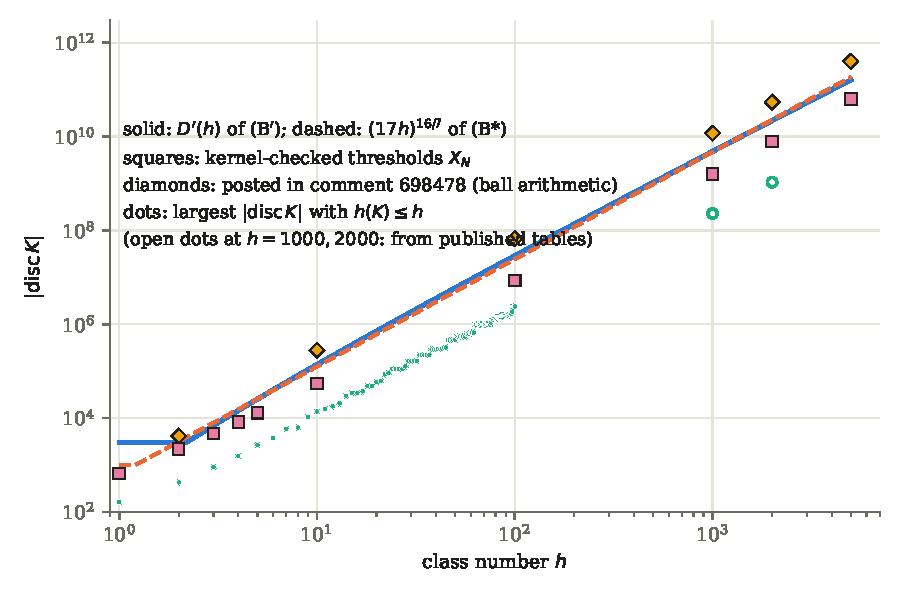
\includegraphics[width=0.92\linewidth]{fig_boundary.pdf}
\caption{Upper bounds for $|\disc K|$ when $h(K) \le h$, on logarithmic axes. Solid: $D'(h)$ of (B$'$). Dashed: $(17h)^{16/7}$, the power form of (B$^*$), which is the minimum of the two. Squares: the ten kernel-checked thresholds. Diamonds: LemmaLab's posted thresholds. Dots: the largest discriminant with class number at most $h$, for $h \le 100$; open dots at $h = 1000$ and $2000$ from the published tables.}
\label{fig:boundary}
\end{figure}

%=====================================================================================================
\section{Calibration against the data}\label{sec:calibration}
%=====================================================================================================

The statements are inequalities about every imaginary quadratic field. We checked them against every field we could compute. None of this is part of the proof.

PARI/GP's \lean{qfbclassno} was run for every fundamental discriminant $-d$ with $5 \le d \le 3\cdot10^6$, $911{,}876$ fields. An independent C program counted reduced forms for every fundamental discriminant with $3 \le d \le 3\cdot10^6$, $911{,}878$ fields. The two agree on the number of fields and the largest $d$ for every $h \le 100$, a range that contains every field with $h \le 100$ by Watkins's theorem.

No field in this range violates any of the statements. The slack is large. Over $d \ge 2981$, $h\log d/\sqrt d$ is at least $2.37$ times $\frac13$ (at $d = 5923$, $h = 7$). Over $d \ge 1000$, $h/d^{7/16}$ is at least $2.52$ times $\frac1{17}$ (at $d = 111{,}763$, $h = 24$). Over $d \ge 5$, $h$ is at most $0.490$ of the bound (U$'$) (at $d = 311$, $h = 19$), and at most $0.558$ of (U$''$) (at $d = 18{,}191$, $h = 213$). Against the largest discriminant with class number at most $h$, (B$^*$) has slack between $6.1$ ($h = 1$) and $13.2$ ($h = 93$), and the thresholds between $3.6$ ($N = 100$) and $5.3$ ($N = 4$), and about $7$ at $N = 1000$ and $2000$ against the published tables. The first version's boundary had slack between $18$ and $63$.

The PARI scripts, the two C programs and the floating-point scripts that recompute every number quoted in \cref{sec:lower,sec:upper,sec:boundary,sec:seveneighths,sec:compare} and in this section are in the entry's directory \lean{numerics/}. Its \lean{README.md} says, for each script, what it checks, what it reads, how to run it and the md5 of its expected output, and \lean{MD5SUMS.txt} (md5 \lean{1ec4f0bd}) lists all sixteen files. Rerun from that directory, every script reproduces its recorded output byte for byte. The figure of \cref{sec:compare} is the one \lean{figure\_v2.py} writes there.

%=====================================================================================================
\section{Verification}\label{sec:verification}
%=====================================================================================================

\subsection{The development}\label{sec:development}

The solution is the library \lean{BoundariesOfClass}, $37$ files and $6{,}513$ lines, in seven parts: \lean{Analytic} (the Gamma ratio near $1$, $\zeta$ near $1$, the per-class minimum), \lean{CS} (Chowla--Selberg at real $\sigma$, the kernel bounds), \lean{Assembly} (one class, the class sums, the uniform bounds and the boundary), \lean{Numerics} (the threshold engine and its instances, (L$'$), (P$'$)), \lean{ClassNumberFormula}, \lean{PolyaVinogradov} and \lean{Primitivity}, and the main module. It contains no \lean{sorry}, \lean{admit}, \lean{native_decide} or \lean{axiom}. The vendored modules are the $75$ \lean{CN1} and \lean{HCN} files of release v1.2.0, unchanged. The published sources differ from those of the run of record in comments only: with comments removed, every published Lean file is identical to the corresponding file in the run of record's tree, and comments in ten files (the main module and nine negative controls) that named internal documents were reworded.

\subsection{The run of record}\label{sec:record}

The checks below ran on 25 October 2026, from 06:54 to 08:33 EDT, in one command of a pinned harness, under a written plan that fixed every check, its expected output and the outcomes that would stop it, before the run. In order:
\begin{enumerate}[nosep]
\item \textbf{Inputs.} The harness's $17$ files and the $58$ specification files were checked against their manifests, and the $76$ vendored source files against the md5s of release v1.2.0. The roots of the audit were set to the challenge's $28$ theorems.
\item \textbf{Static gate.} The $37$ solution files and $75$ vendored files passed a static gate over the sources and the $142$ built modules, recorded in a manifest of $113$ source files.
\item \textbf{Extension check.} The environment extensions of all $112$ audited compiled modules were inspected for initializers, elaborators and instances.
\item \textbf{Recompilation.} Every one of the $112$ audited modules was recompiled from source with plain \lean{lean}, and all $112$ compiled files were byte-identical to the ones the later checks read.
\item \textbf{Comparator} (\cref{sec:comparator}).
\item \textbf{The closure audit} of each of the $28$ roots, each followed by a post-check of its output (\cref{sec:audit}).
\item \textbf{Re-verification.} At the end, none of the $112$ compiled files had changed.
\end{enumerate}
Every stage passed, and the harness printed its final verdict line. An earlier dry run on the same inputs agrees with the run of record in every recorded result: closure sizes, edges, module sets and axioms.

\subsection{Comparator}\label{sec:comparator}

Comparator \cite{Comparator}, with the challenge module \lean{BoundariesOfClassChallenges.BoundaryV2}, the solution module \lean{BoundariesOfClass.Main}, the $28$ theorem names, the three permitted axioms and nanoda enabled, reported
\begin{center}
``nanoda kernel accepts the solution'', \quad ``Lean default kernel accepts the solution'', \quad ``Your solution is okay!''
\end{center}
in about eight minutes. The binary is a copy of Comparator \lean{v4.34.0} with one patched hunk: where Comparator would call \lean{lake build}, it refuses unless the compiled module already exists. Before it ran, a wrapper checked that the challenge, recompiled with plain \lean{lean}, gives a compiled file byte-identical to the one Comparator reads; that no audited compiled file had changed since the recompilation step; and that the Lean search path equals a pinned list of twelve entries. The binaries are the patched Comparator \lean{2da1112f}, lean4export \lean{b8b81a76} and nanoda \lean{f6268f7a} (md5 prefixes); the last two are the ones used for the earlier entries.

\subsection{The closure audit}\label{sec:audit}

A closure walk from each of the $28$ theorems follows types, the values of theorems, definitions and opaque constants, inductive types with their constructors and recursors. It does not read the axiom cache of the compiled modules. All $28$ pass.
\begin{itemize}[nosep]
\item \textbf{Size.} The closures have between $43{,}787$ constants (the Pólya--Vinogradov inequality) and $129{,}020$ (the boundary (B$^*$)).
\item \textbf{Axioms.} Exactly \lean{propext}, \lean{Classical.choice} and \lean{Quot.sound} in every closure, with no \lean{sorryAx}, no \lean{Lean.ofReduceBool} and no unsafe or partial constant.
\item \textbf{The $7/8$ theorem, at real points only.} In the $17$ roots for the lower bounds, (P$'$), the two boundaries and the thirteen thresholds, the closure contains the $26{,}740$ constants of openai/math's $7/8$ development, and the set of references from a constant outside openai/math to a constant inside it is exactly one: \lean{CN1.LFunction_ofReal_re_pos_of_seven_eighths_lt} referring to \lean{OAI.DirichletCharacter.LFunction_ne_zero_of_seven_eighths_lt_re}, applied at the image of a real number. So OpenAI's theorem is used only through the sign of $L(\sigma,\chi)$ at real $\sigma$.
\item \textbf{No zero-free region in the upper bounds.} The closures of the other $11$ roots, the class number formula, (L1), (U$'$), (U$''$), Pólya--Vinogradov, the half-log bounds, uniqueness and primitivity, contain no constant of openai/math, of PrimeNumberTheoremAnd or RellichKondrachov, or of the second paper's \lean{HCN} modules.
\item \textbf{No class-number tables.} The lower-bound closures draw their first-project and second-paper constants only from an allowlist of modules fixed in the plan, which excludes the earlier proofs' finite-range certificates and main theorems and any constant whose type fixes a class number; the upper-bound closures have a stricter allowlist. No root has a disallowed module or a forbidden import.
\end{itemize}

\subsection{Controls}\label{sec:controls}

A checker that accepts everything is worthless, so the harness carries controls that must fail. Each was run with the harness, and rerun by the separate review (\cref{sec:replay}), and each failed as required.
\begin{enumerate}[label=(\alph*),nosep]
\item The challenge with one threshold tampered, $660 \to 661$: ``statement do not match''.
\item A false lemma admitted by switching off the elaborator's kernel check (\lean{debug.skipKernelTC}): rejected by nanoda and by Lean's kernel with nanoda on, and by Lean's kernel alone with nanoda off.
\item A proof by \lean{sorry}: ``Illegal axiom detected: \lean{sorryAx}''.
\item A missing compiled solution module, a stale compiled challenge, and an inherited Lean search path: each refused before Comparator ran. A search path with one pinned entry dropped was refused after the other checks passed.
\item The static gate on a crafted fixture, eleven corruptions of the inputs, thirteen corruptions of audit outputs, and two aborted stages: each refused or failed as specified, and an aborted stage left nothing later run.
\end{enumerate}
The development also contains, outside the solution library, Lean proofs that tampered statements are false at real fields (for example at $K = \Q(\sqrt{-163})$ and $\Q(\sqrt{-427})$, using the earlier entries' theorems), and that tampered constants such as $\frac38$ in (L$'$), $\frac1{14}$ in (P$'$) or $X'_2 = 2190$ cannot be derived from the threshold engine at real fundamental discriminants. These were built, but are not part of the run of record.

\subsection{The replay by a separate session}\label{sec:replay}

A separate AI review session, not one of the sessions that wrote the proof, reran the whole pinned command from its own verified copies of the harness and specifications on the same day, from 08:35 to 10:10 EDT. It ended with the same verdict, and a field-by-field comparison of its $31$ result files with the run of record, run-specific fields such as timestamps excluded, found no differences. The $28$ post-check outputs and the Comparator configuration are byte-identical. The comparison script was itself checked: on a copy of the run of record with four planted changes it reported exactly those four. The review reran every control suite from its own copy, and each passed. It disclosed one error of its own: its first attempt at the search-path control was invalid, because its wrapper's search path lacked a system directory and the control refused for the wrong reason; only the rerun with the harness's own path counts.

This replay adds an independent execution, not independent tooling. The review's harness is byte-identical to the run of record's by design, the machine, toolchain and package directory are the same, and the dependencies were not rebuilt. A fresh clone closes the gap of the shared package directory. On 3 November 2026 the published repository was cloned from GitHub (the release branch, before tagging) and the entry was built by its README's instructions, in an empty directory with its own package store. The pinned packages were cloned and patched, the Mathlib cache was downloaded, the six libraries were built, and the patches were re-verified. Comparator then reported, again, that nanoda and Lean's kernel accept all $28$ theorems. That run used the same machine and the same Comparator, lean4export and nanoda binaries, so it does not close the gap of the machine; a replay elsewhere would. A separate AI review session repeated the fresh build from its own copy of the published tree, in its own directory with its own package store and its own download of the Mathlib cache, and Comparator (the same binaries and configuration) again reported that nanoda and Lean's kernel accept all $28$ theorems. The review is an AI review, not a referee's report.

\subsection{Caveats}\label{sec:caveats}

The runs are local and unsandboxed. The sandboxing layer that Comparator normally uses was replaced by a pass-through shim, because the machine runs macOS; the static gate, the extension check and the recompilation run first, and the run aborts if any fails. The compiled dependency files of openai/math, Mathlib and the other packages come from a local package directory shared with the earlier entries, and were not rebuilt for this run; Comparator's export and its two kernel replays re-check the exported closure, the dependencies included.

\subsection{The author's check}\label{sec:authorcheck}

The author read back the paper and the verification record on 2 November 2026, and approved them.

%=====================================================================================================
\section{What we do and do not claim}\label{sec:notclaimed}
%=====================================================================================================

We claim a kernel-checked proof of the $28$ statements of \cref{app:statements}, by the routes of \cref{sec:route}, with the record of \cref{sec:verification}. We do not claim the mathematics: the lower bound is the Gronwall--Hecke deduction \cite{Landau1918} with OpenAI's theorem \cite{OAIqrh} as input, along LemmaLab's class-sum route; the upper bounds are Dirichlet's, Pólya's and Vinogradov's. We do not claim priority among formalizations of results of this kind.

The lower bounds rest on openai/math's theorem that Dirichlet $L$-functions do not vanish for $\re s > 7/8$. As far as we know its manuscript is not refereed. Its Lean proof is inside the checked closure, so the kernels have checked it; what a human reader may want, and does not yet have, is a refereed understanding of why it is true. The theorem is used at real points only. Any input that excludes real zeros of $L(s,\chi_{-d})$ in $[7/8, 1)$ would serve, with the same constants. The upper bounds use no zero-free region.

Nothing here bears on the Riemann hypothesis, or on Siegel zeros beyond what the $7/8$ theorem itself gives. This development proves nothing new about zeros of $L$-functions.

The comparisons of \cref{sec:compare} are as of the sources we read, on the dates given. At class number one the bounds here are not the best known; at two points our own evaluation of Jaswal's method, which he did not post, is better than our kernel-checked statements; and for very large $d$ the bound zeta-lab obtains from the full half-plane is better than ours (\cref{sec:positioning}). A threshold is not a classification: turning these thresholds into complete lists of fields of small class number is future work.

The statements bound $d$ from above. They say nothing about the existence of fields of class number $h$ near the bounds, about real quadratic fields, or about orders that are not maximal.

Finally, this paper describes the mathematics and the checking. It is not itself checked by anything. Where it says what a Lean declaration states, the declaration is the authority.

%=====================================================================================================
\section*{Acknowledgments and AI disclosure}
%=====================================================================================================

The quasi-Riemann hypothesis at $7/8$ for all Dirichlet $L$-functions, with its Lean proof, is OpenAI's (openai/math, family 003, Apache-2.0). The deduction of class number bounds from zero-free segments is Gronwall's and Hecke's, as published by Landau. The class number formula is Dirichlet's, and the character-sum inequality is Pólya's and Vinogradov's. The challenge is Terence Tao's. The Chowla--Selberg formula is S.~Chowla's and A.~Selberg's \cite{ChowlaSelberg1967}. In the comments of Tao's post, michaelmross gave the expansion of the principal form by Poisson summation (comment 698466); Tao observed that with the $7/8$ theorem it gives $d < 655$ (comment 698471); LemmaLab evaluated it at $s = 7/8$ and certified $d \le 653$ (comment 698472), extended the argument to all class numbers with posted thresholds (comment 698478), and stated the $d^{3/8}/12$ form of the bound at $7/8$ (comment 698484). This paper's lower bounds follow that extension, with each class charged its exact minimum. Manvir Jaswal's paper, linked from an anonymous comment (698561), is the source of the Hecke-integral bound we compare against; Iwao Kimura's of the explicit zero gap and the Lean-checked thresholds.

The commenters and authors state their own use of AI, which we record as they give it. michaelmross developed his lemma, its proof and his scripts with Claude Opus (Anthropic). Tao's observation came from playing with the SAIR open model. LemmaLab worked with Claude (Anthropic), and had the class-number-one bound re-checked independently with ChatGPT (comment 698472) and the extension to all class numbers and its applications with Codex (comments 698478 and 698484), both OpenAI's. Nielsen's Lean proof of the completeness of Euler's convenient numbers (comment 698545) was produced by Codex. Jaswal writes: ``This paper was produced by a multi-agent AI research system that the author built and ran, using Anthropic Claude Opus 5.5: apart from the work of others that it cites, the ideas, proofs, computations and text are due to the system'' \cite{Jaswal2026}; the comment that links it says that ``Claude helped draft this comment''. Kimura states that the explicit argument, the Lean files, the sieve and most of the text were done with Claude Opus 5.5 (Anthropic) through Claude Code, under his direction \cite[\S8]{Kimura2026}.

We thank Mathlib and its contributors for the number-field, class-group, discriminant, Dedekind zeta and residue (X.~Roblot), $L$-series, Gauss sum (M.~Stoll), discrete Fourier transform and primitive-character (D.~Loeffler), Gamma and zeta infrastructure the development leans on throughout; the authors of the packages OpenAI's proof builds on, including PrimeNumberTheoremAnd \cite{PNT} and RellichKondrachov \cite{RK}; Chris Bailey for nanoda, the second kernel; and the authors of Comparator and lean4export, the checking pipeline.

The formalization, the numerics, the calibration code and this paper were produced with extensive use of an AI assistant (Claude, Anthropic) under the direction of the author, in separate sessions. A separate AI session reviewed the plan, the statements and the delivered parts, and reproduced the run of record from its own copies (\cref{sec:replay}). The mathematical routes are due to the people credited above. The Lean kernel is the trusted component. The history, the attributions, the comparisons and the account of how the work was checked are ours, and we have tried to say how each was obtained.

\bibliographystyle{amsplain}
\bibliography{refs}

\appendix
\section{The 28 statements, verbatim}\label{app:statements}

The theorem declarations of the challenge module \lean{BoundariesOfClassChallenges.BoundaryV2}, whose source file has md5
\begin{center}\lean{fc55db128ee8596029634ec52e9dea15},\end{center}
in the order of the file, with their docstrings and the section headers removed and nothing else changed. They live in the namespace \lean{BoundariesOfClass}, with \lean{open NumberField}.

\lstinputlisting{statements_v2_extract.lean}

\end{document}
